\section{Infraestrutura de Chaves Públicas Brasileira}

A Infraestrutura de Chaves Públicas Brasileira, mais comumente conhecida por ICP-Brasil, é a cadeia hierárquica regulamentada  responsável pela emissão de certificados digitais no Brasil. Criada em 2001 pela Medida Provisória 2.200-2, a ICP-Brasil surge com a finalidade de normatizar e estabelecer os requisitos técnicos necessários para realizar a identificação virtual de entidades e de cidadãos brasileiros.

O Instituto Nacional de Tecnologia da Informação (ITI) é a autarquia federal responsável por operar e supervisionar a ICP-Brasil a fim de garantir sua segurança. Ao ITI compete a responsabilidade de fiscalizar, credenciar, descredenciar as demais entidades da cadeia, além de ser a Autoridade Certificadora Raiz, a qual executa as Políticas de Certificados, emite, expede, distribui, revoga e gerencia os certificados das autoridades certificadoras imediatamente abaixo \cite{ICPBrasi30}.

À AC Raiz estão credenciadas as Autoridades Cerificadoras, cujo objetivo é gerenciar os certificados digitais associando pares de chaves criptográficas ao seu titular, podendo ser uma outra AC ou um usuário final. A Figura \ref{hierarquia} descreve de forma detalhada cada nível da hierarquia da ICP-Brasil.

\begin{figure}[h]
	\centering
	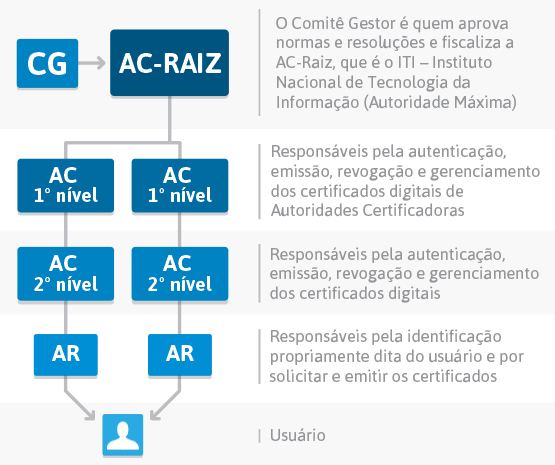
\includegraphics[keepaspectratio=true,scale=0.6]{figuras/hierarquia ICP-Brasil.png}
	\caption{Hierarquia da ICP-Brasil \cite{hierarquiaICP}.}
	\label{hierarquia}
\end{figure}

 